\documentclass[t]{beamer}

\mode<presentation>
{
  \usetheme{default}
  \setbeamertemplate{navigation symbols}{}
  \setbeamertemplate{footline}[frame number]
  \setbeamertemplate{items}[circle]
  \usecolortheme{seahorse}
}

\usepackage[english]{babel}
\usepackage[utf8]{inputenc}
\usepackage{times}
\usepackage[T1]{fontenc}
\usepackage{url}
\usepackage{amsmath}

\parskip=8 pt

\newcommand\topstrut{\rule{0pt}{2.6ex}}
\newcommand\bottomstrut{\rule[-1.2ex]{0pt}{0pt}}
\newcommand\doublestrut{\rule[-1.2ex]{0pt}{3.6ex}}

\newcommand\blue[1]{\textcolor{blue}{#1}}
\newcommand\red[1]{\textcolor{red}{#1}}
\newcommand\gray[1]{\textcolor{gray}{#1}}
\newcommand\smallgray[1]{\textcolor{gray}{\small\it #1}}
\newcommand\prevwork[1]{\smallgray{#1}}

\title
{Statistics for Machine Learning and Big Data}
\subtitle{An Introduction}

\author[Abrahamson] {Jeff Abrahamson}

% Delete this, if you do not want the table of contents to pop up at
% the beginning of each subsection:
\AtBeginSubsection[]
{
  \begin{frame}<beamer>{Outline}
    \tableofcontents[currentsection,currentsubsection]
  \end{frame}
}

% If you wish to uncover everything in a step-wise fashion, uncomment
% the following command: 
%\beamerdefaultoverlayspecification{<+->}

\begin{document}

\begin{frame}
  \titlepage
\end{frame}

\begin{frame}
  \frametitle{Outline}
  \tableofcontents
\end{frame}

\section{Probability}

\begin{frame}
  \frametitle{Review}
  \begin{itemize}
  \item Counting
  \item Urns (sampling)
  \item Area
  \end{itemize}
\end{frame}

\begin{frame}
  \frametitle{}

\end{frame}

\begin{frame}
  \frametitle{Counting}

  Example: two children, what is $P(\exists \mathrm{boy}) = P(\exists b)$?
  \only<2>{graphic of bb, bg, gb, gg with prob 1/4}
  \only<3->{graphic of bb, bg, gb, gg with prob 1/4 with circled if $\exists$ b}
  \only<4->{What about $P(\exists b \mid \exists g)$?}
  \only<5->{same graphic, fade bb, circles, show 2/3}
  \only<6->{Events have probabilities summing to 1, cover, and are disjoint.}
\end{frame}

\begin{frame}
  \frametitle{Pólya urn model}

  $r$ red balls, $b$ black balls in an urn.

  \only<2->{
  \begin{itemize}
  \item Sampling with replacement and duplication (rich get richer)
  \item Variations: balls into boxes
    \begin{itemize}
    \item Sampling with replacement
    \item Sampling without replacement
    \end{itemize}
  \end{itemize}
  }
  \only<3->{Want to know sequence of colours selected, evolution of colour distribution in urn.}
\end{frame}

\begin{frame}
  \frametitle{Sampling}

  \begin{itemize}
  \item We don't know $r$, $b$, or even $r/b$.  Estimate.
  \end{itemize}

  % http://en.wikipedia.org/wiki/Simple_random_sample
  % http://en.wikipedia.org/wiki/Urn_problem
\end{frame}

\begin{frame}
  \frametitle{Area}

  \begin{itemize}
  \item Continuous case.
  \item Events are regions.
  \item Same constraints: sum of areas is unity.  Cover and disjoint.
  \item Zero probability events!
  \end{itemize}
\end{frame}

\begin{frame}
  \frametitle{Distributions}

  Sneak preview of some common distributions, what they look like, and processes giving rise to them.
\end{frame}


\section{Statistics}
%\subsection{Subsection}

\begin{frame}
  \frametitle{What is statistics?}
  \begin{enumerate}
  \item<1-> Identify a question or problem.
  \item<1-> Collect relevant data on the topic.
  \item<1-> Analyze the data.
  \item<1-> Form a conclusion.
  \end{enumerate}
  \only<2>{Sadly, sometimes people forget 1.}
  \only<3->{Statistics is about making 2--4 efficient, rigorous, and meaningful.}
  \only<4>{\prevwork{\textit{OpenIntro Statistics}, 2nd edition, D.~Diez, C.~Barr, M.~Çetinkaya-Rundel, 2013.}}
\end{frame}


\begin{frame}
  \frametitle{Significance}

  \begin{itemize}
  \item Flip a coin $N$ times.  Get 49\% heads.  Is the coin fair?
  \item Congress/parliament has $N$ members of whom $m$ are male.  Do
    we discriminate against women?
  \item Do we discriminate against women more or less than we
    discriminate against blacks?
  \item Email classification: spam or not?
  \item Careful about what we conclude.  Here we can't conclude
    anything about cause or source.
  \end{itemize}

  % This needs supporting slides with computations.  We'll also have
  % to come back to it when we understand about $p$ values and the
  % like.
  
\end{frame}

\begin{frame}
  \frametitle{Terminology}

  \begin{itemize}
  \item A \textbf{case} or {observational unit} is an observation or a
    single sample.  E.g., an email.
  \item A \textbf{variable} is a characteristic of an observational
    unit.  E.g., number of lines, mean line length, number of words.
  \end{itemize}
  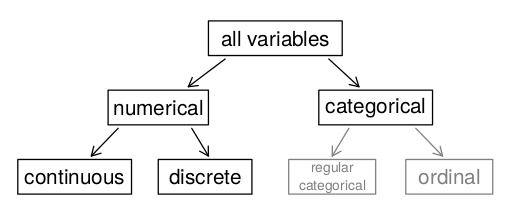
\includegraphics[width=.9\textwidth]{variable-types.png}

  Notes:  Categorical is sometimes called nominal.  Categorical
  variables with logical ordering (empty, half, full) or called ordinal.
\end{frame}

\begin{frame}
  \frametitle{Anecdote}

  Some properties of anecdote:
  
  \begin{itemize}
  \item is data
  \item haphazardly collected
  \item is generally not representative
  \item sometimes result of selective retention
  \item does not accumulate to be representative
  \item might be true (by chance)
  \item is ok to use as hypothesis, but be clear that hypothesis is anecdote
  \end{itemize}
\end{frame}

\begin{frame}
  \frametitle{Simple random sample}

  Uniform and independent.

  The gremlins:
  \begin{itemize}
  \item Not actually random
  \item Convenience sample
  \item Non-response bias
  \end{itemize}

\end{frame}

\begin{frame}
  \frametitle{}

\end{frame}

\begin{frame}
  \frametitle{}

\end{frame}

\begin{frame}
  \frametitle{}

\end{frame}

\begin{frame}
  \frametitle{}

\end{frame}

\begin{frame}
  \frametitle{}

\end{frame}

\begin{frame}
  \frametitle{}

\end{frame}

\begin{frame}
  \frametitle{}

\end{frame}

\begin{frame}
  \frametitle{}

\end{frame}

\begin{frame}
  \frametitle{}

\end{frame}

\begin{frame}
  \frametitle{}

\end{frame}

\begin{frame}
  \frametitle{}

\end{frame}

\begin{frame}
  \frametitle{}

\end{frame}

\begin{frame}
  \frametitle{}

\end{frame}

\begin{frame}
  \frametitle{}

\end{frame}

\begin{frame}
  \frametitle{}

\end{frame}

\begin{frame}
  \frametitle{}

\end{frame}

\begin{frame}
  \frametitle{}

\end{frame}

\begin{frame}
  \frametitle{}

\end{frame}

\begin{frame}
  \frametitle{}

\end{frame}

\begin{frame}
  \frametitle{}

\end{frame}

\begin{frame}
  \frametitle{}

\end{frame}

\begin{frame}
  \frametitle{}

\end{frame}

\begin{frame}
  \frametitle{Questions?}
  \vspace{3cm}
  \centerline{\large\url{purple.com/talk-feedback}}
\end{frame}


\end{document}
